\subsection{Learning Subconscious Behaviours}
\label{sub:sec:solution:WoZ}

Both \ac{ML}-based modules proposed in Section~\ref{sub:sec:solution:arch} need to be trained in order to learn how to generate correct backchannels. Note, as mention in Section~\ref{subsec:RestrictedPerceptionsWOZStudy}, that in \ac{WoZ} the human subject is not aware that the agent is being controlled manually (partially or fully) by another human, the wizard. In the traditional \ac{WoZ}, the wizards have full access to what is happening in the scenario and have control over the virtual agent, using a \ac{UI}. However, as aforementioned by Sequeira et al., it is relevant to take into account that the virtual agent has inherent limitations in their perceptional abilities and their actions onto their external world~\cite{Sequeira2016}. Moreover, social behaviours are mostly done subconsciously, therefore, the experiment could be influencing the results by just forcing the user to rationalise over what is being subconsciously felt. Taking this two issues into account, we propose an approach for learning correct backchannel generation in virtual agents and embodied agents in \ac{HRI} using limited-perception \ac{WoZ} and human experts for corrective feedback (Figure~\ref{fig:learning:process}).



\begin{figure}
	\centering
	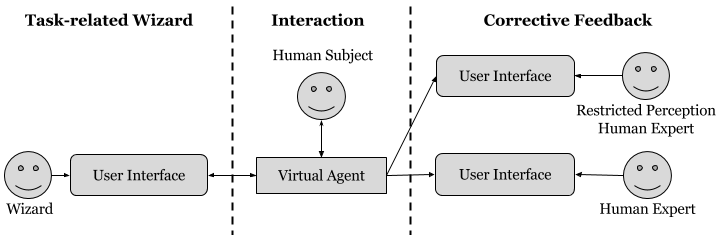
\includegraphics[width=\textwidth]{images/CorrectiveFeedbackRestrictiveWoZ_Diagram.png}
	\caption{Using perceptual readings and limited perception \ac{WoZ} to assess backchannels quality. Human experts monitor the interaction and provide corrective feedback according to their perceptions. The task-related wizard is optional.}
	\label{fig:learning:process}
\end{figure}

Following Figure~\ref{fig:learning:process}, one wizard is responsible for controlling the virtual agents task-related actions and two human experts for providing corrective feedback regarding whether the agent's behaviour is socially appropriate or inappropriate~\cite{Kok2012, Poppe2011}, using a \ac{UI}. One human expert will have its perceptions limited with same extent as the virtual agent, and the other will have unrestricted perceptions. This approach can be seen as reverse-\ac{RL} since it is possible to map the human experts feedback to a reward function, in which, appropriate and inappropriate backchannels will have values values $1$ and $-1$, respectively.

Using this approach it is possible to obtain multiple feedback over the generated behaviours, similar to \ac{PCS}~\cite{Huang2010} without influencing the results by forcing the users to rationalise their actions. Cohen's kappa coefficient $\kappa$ may be used to measure inter-rated agreement between two human experts (Equation~\ref{eq:CohenKappa}). In the equation, $p_0$ is the relative observed agreement and $p_e$ the probability of random agreement.


\vspace{-3mm}
\begin{equation}
	\label{eq:CohenKappa}
	\kappa = \frac{p_0 - p_e}{1 - p_e}
\end{equation}

With the data collected using the restricted-perception \ac{WoZ}, the data will be pre-processed and used to train the \ac{ML}-based component using Weka~\cite{Hall2009}. \ac{RL} algorithms will take priority since they were the main suggestion from several authors~\cite{Thomaz2006, Kok2012, Zhao2014, Papangelis2014, Blumberg2002, Andrist2015, Mutlu2006}. Nevertheless, similar approaches can be further investigated. 

As summarised in equation~\ref{eq:IterativeSolutionEquation}, the system evolves as follows. The initial version $M_0$ is the only version that is strictly rule-based and stripped of previous knowledge according to the information collected from preliminary studies, and the interactional goals. The goal of $M_0$ is to explore as many state combinations as possible in order to produce great number of backchannels, and acquire, as much corrective feedback as possible from the human experts~\cite{Kok2012}. The corrective feedback collected on $M_n$ is later used to train $M_{n+1}$ version of the rapport agent. Following this pattern, we expect $M_n$ to build better rapport than the previous $M_{n-1}$ version. Note that, after the first learning state, the initial excessive backchannels rules must be discarded and replaced by the \ac{ML} generated backchannels, similar to how \ac{IPL} (Section~\ref{subsec:IterativePerceptualLearning}) discards the negative samples after the first subjective evaluations. 

\vspace{-3mm}
\begin{equation}
	\label{eq:IterativeSolutionEquation}
	M_{n+1} = M_{n} + Corrective\, Feedback
\end{equation}

To conclude, after several iterations~\cite{Sequeira2016, Kok2012}, the best possible model $M_n$ will be one tested on users, in which human experts are not required to be present since the agent does not benefit from further training. The final system should represent the average listener's behaviour interacting with the average speaker. Preliminary studies may be conducted to assess the feasibility of the proposed learning strategy.